\documentclass{NEXT-SCNUThesis}

\title{SCNUThesis}
\author{郑誉}
\studentid{20210000000}
\majorclass{xxx}
\supervisor{xxx}
\date{2025年4月}

\keywordsen{Transformer; Attention; Neural Network}
\keywordszh{变换器, 注意力, 神经网络}

\begin{document}
    \maketitle

    \begin{abstracten}
        The abstract in English goes here. Abstract in English and that in
        Chinese presented on the previous page should agree. This section provides
        a concise summary of the research, including objectives, methods,
        results, and conclusions.

        Transformer is a neural network architecture that relies on self-attention
        mechanisms to draw global dependencies between input and output. Unlike
        previous sequence-to-sequence models, the Transformer does not require that
        the sequence be processed in order.
    \end{abstracten}

    \begin{abstractzh}
        中文摘要在这里。中文摘要和英文摘要应该一致。该部分提供了研究的简要总结,包括目标、方法、结果和结论。

        变换器是一种神经网络架构,依赖于自注意力机制来绘制输入和输出之间的全局依赖关系。与以前的序列到序列模型不同,变换器不需要按顺序处理序列。
        变换器的主要优点是并行处理序列数据,从而加快训练速度。它在自然语言处理、计算机视觉等领域取得了显著的成功。
    \end{abstractzh}

    \toc

    \chapter{MAIN BODY}

    \section{Figures}
    \subsection{Example A}
    This is an example of the Fig~\ref{fig:example-figure} citation.

    \begin{figure}[htbp]
        \centering
        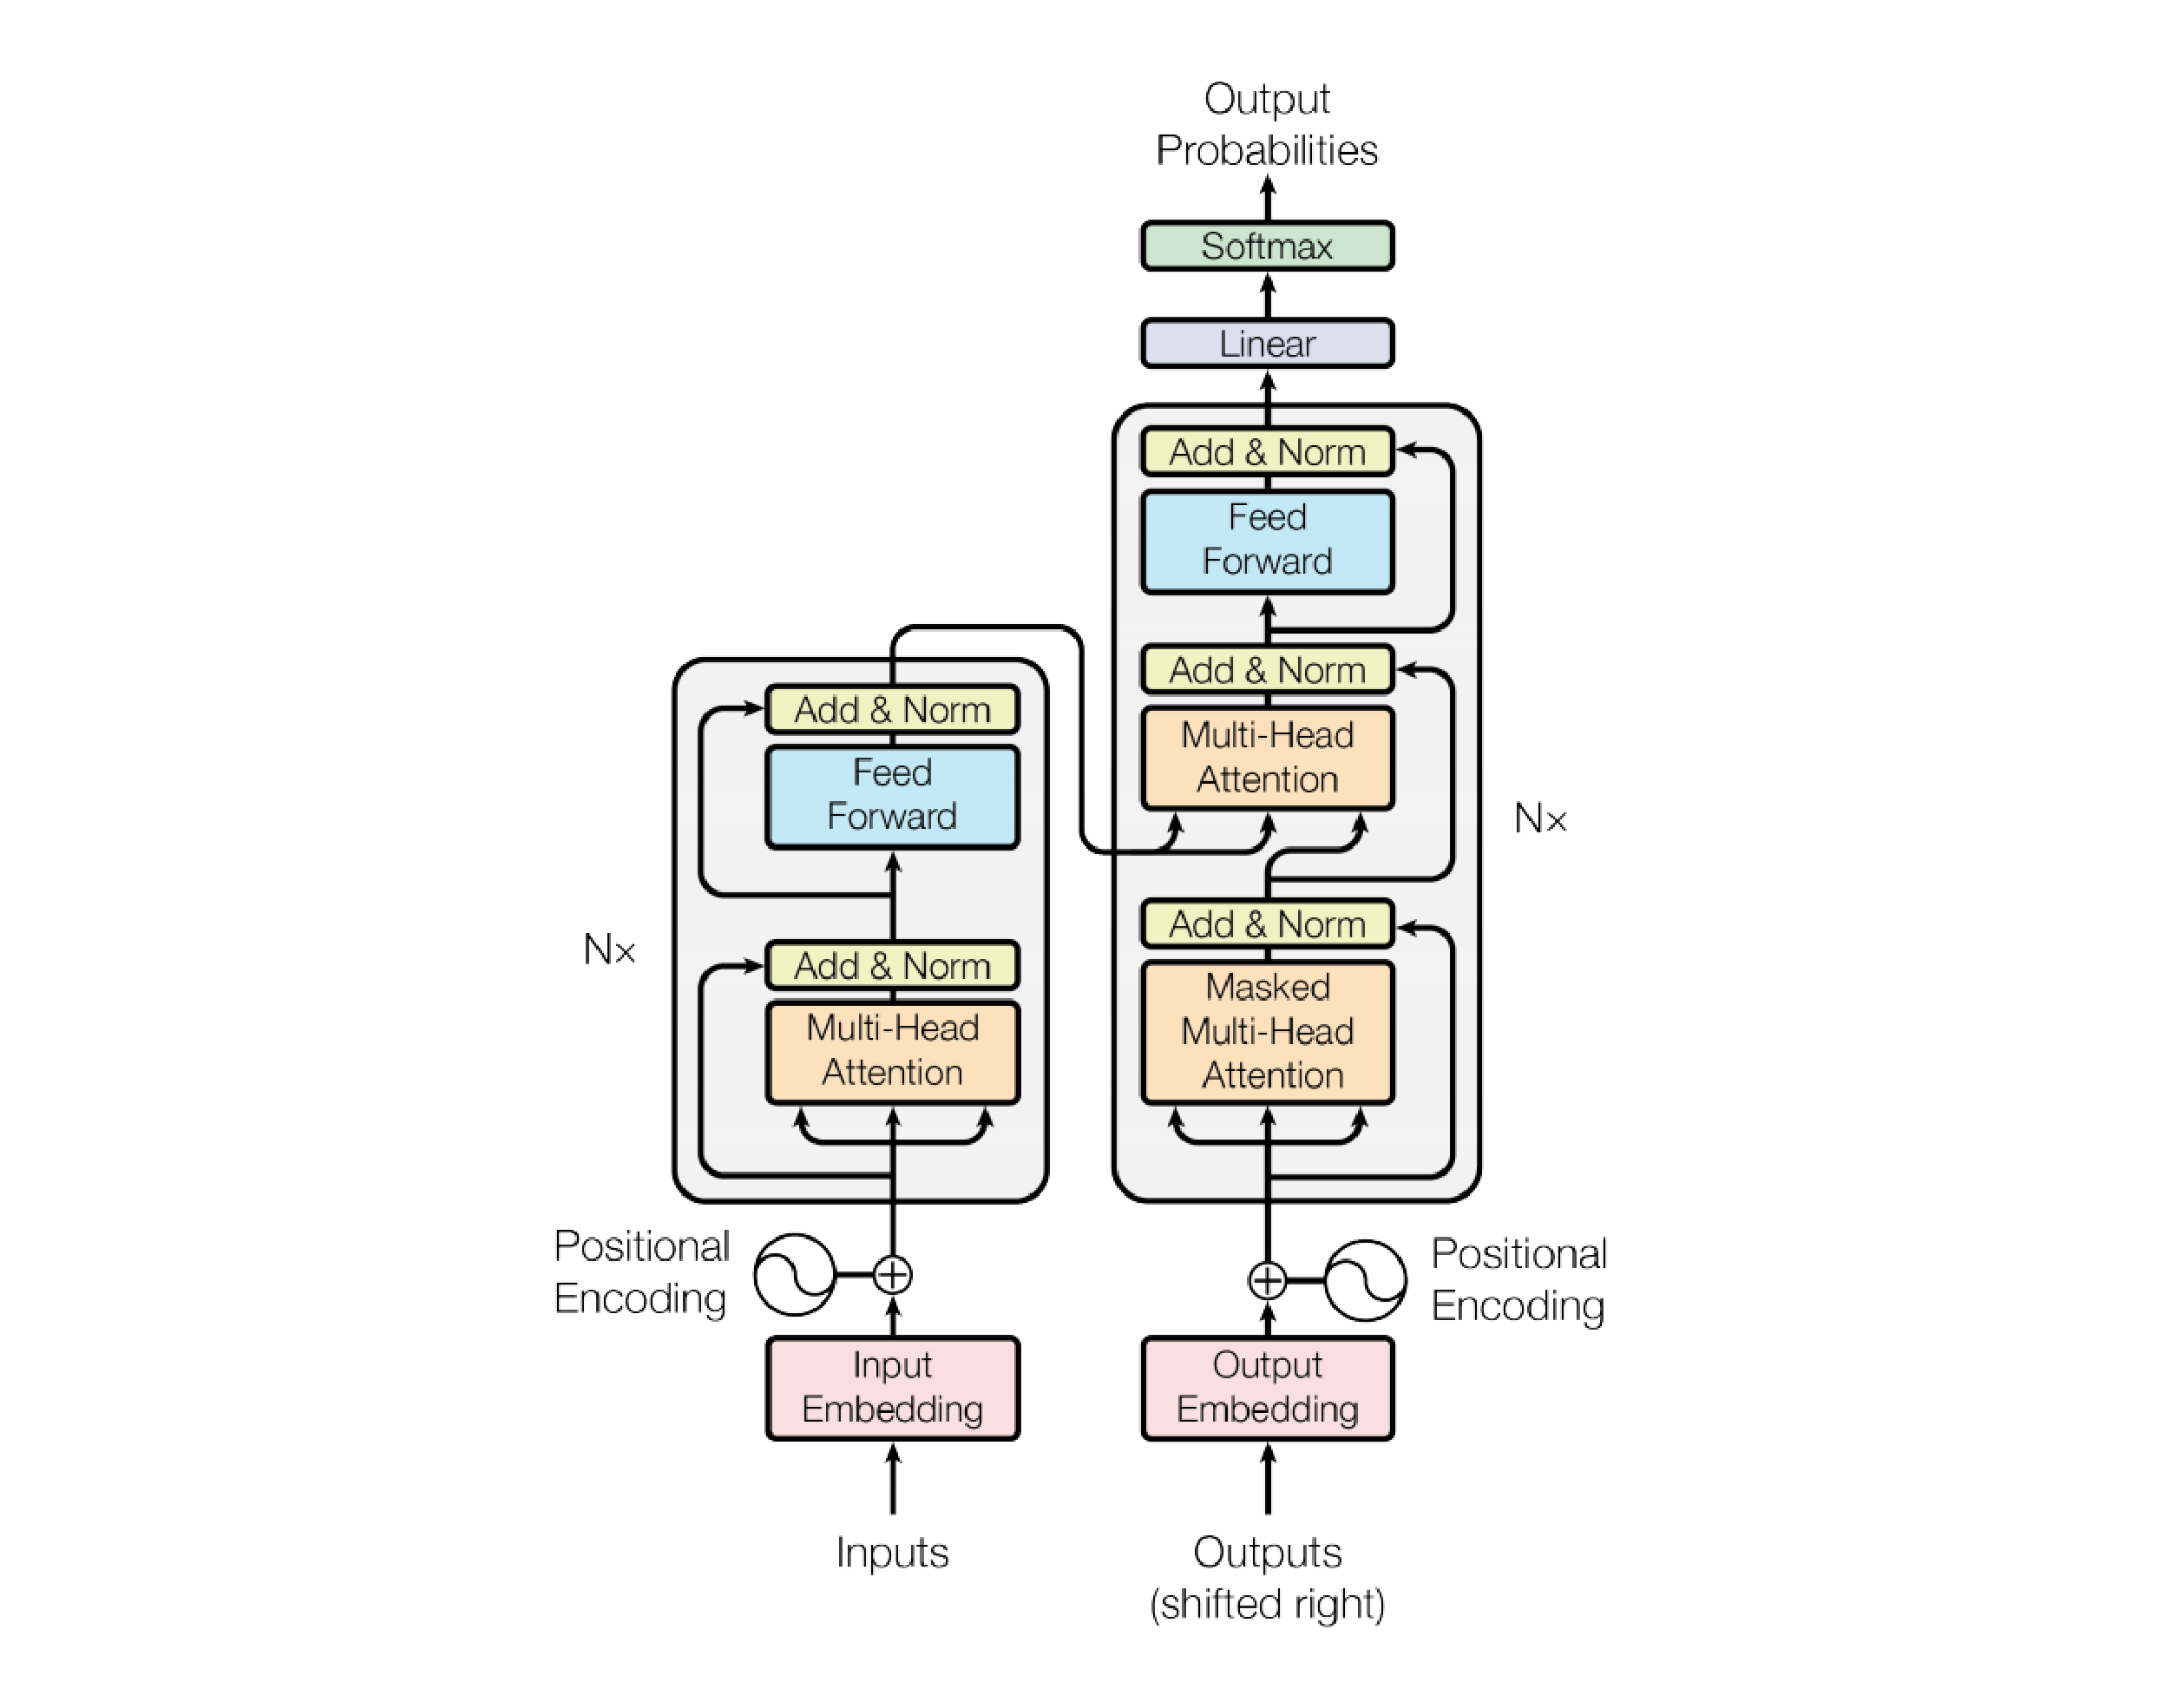
\includegraphics[width=0.5\textwidth]{fig/transformer.eps}
        \caption{Example figure}
        \label{fig:example-figure}
    \end{figure}

    \section{Tables}
    \subsection{Example A}
    This is an example of the Table~\ref{tab:example-table} citation.
    \begin{table}[htbp]
        \centering
        \caption{Example table}
        \label{tab:example-table}
        \begin{tabular}{|c|c|}
            \toprule Column 1 & Column 2 \\
            \midrule Row 1    & Row 2    \\
            Row 3             & Row 4    \\
            \bottomrule
        \end{tabular}
    \end{table}

    \section{Equations}
    \subsection{Example A}
    This is an example of the inline equation $E=mc^{2}$.
    \subsection{Example B}
    This is an example of the equation
    \begin{equation}
        E=mc^{2}
    \end{equation}

    \section{Citation}
    You can cite references in the text using the \texttt{cite} command.
    \subsection{Example A}
    This is an example of a citation
    $\backslash cite\{vaswaniAttentionAllYou2017\}$
    \cite{vaswaniAttentionAllYou2017}.
    \subsection{Example B}
    This is an example of a citation $\backslash cite\{girshickFastRCNN2015\}$ \cite{girshickFastRCNN2015}.

    \chapter{正文}

    \reference{reference}
    \appendix
    \section{Appendix A}
    \section{Appendix B}
    \section{Appendix C}

    \acknowledgements
\end{document}